\documentclass[11pt]{article}\usepackage[]{graphicx}\usepackage[]{color}
%% maxwidth is the original width if it is less than linewidth
%% otherwise use linewidth (to make sure the graphics do not exceed the margin)
\makeatletter
\def\maxwidth{ %
  \ifdim\Gin@nat@width>\linewidth
    \linewidth
  \else
    \Gin@nat@width
  \fi
}
\makeatother

\definecolor{fgcolor}{rgb}{0.345, 0.345, 0.345}
\newcommand{\hlnum}[1]{\textcolor[rgb]{0.686,0.059,0.569}{#1}}%
\newcommand{\hlstr}[1]{\textcolor[rgb]{0.192,0.494,0.8}{#1}}%
\newcommand{\hlcom}[1]{\textcolor[rgb]{0.678,0.584,0.686}{\textit{#1}}}%
\newcommand{\hlopt}[1]{\textcolor[rgb]{0,0,0}{#1}}%
\newcommand{\hlstd}[1]{\textcolor[rgb]{0.345,0.345,0.345}{#1}}%
\newcommand{\hlkwa}[1]{\textcolor[rgb]{0.161,0.373,0.58}{\textbf{#1}}}%
\newcommand{\hlkwb}[1]{\textcolor[rgb]{0.69,0.353,0.396}{#1}}%
\newcommand{\hlkwc}[1]{\textcolor[rgb]{0.333,0.667,0.333}{#1}}%
\newcommand{\hlkwd}[1]{\textcolor[rgb]{0.737,0.353,0.396}{\textbf{#1}}}%
\let\hlipl\hlkwb

\usepackage{ulem}

\usepackage{framed}
\makeatletter
\newenvironment{kframe}{%
 \def\at@end@of@kframe{}%
 \ifinner\ifhmode%
  \def\at@end@of@kframe{\end{minipage}}%
  \begin{minipage}{\columnwidth}%
 \fi\fi%
 \def\FrameCommand##1{\hskip\@totalleftmargin \hskip-\fboxsep
 \colorbox{shadecolor}{##1}\hskip-\fboxsep
     % There is no \\@totalrightmargin, so:
     \hskip-\linewidth \hskip-\@totalleftmargin \hskip\columnwidth}%
 \MakeFramed {\advance\hsize-\width
   \@totalleftmargin\z@ \linewidth\hsize
   \@setminipage}}%
 {\par\unskip\endMakeFramed%
 \at@end@of@kframe}
\makeatother

\definecolor{shadecolor}{rgb}{.97, .97, .97}
\definecolor{messagecolor}{rgb}{0, 0, 0}
\definecolor{warningcolor}{rgb}{1, 0, 1}
\definecolor{errorcolor}{rgb}{1, 0, 0}
\newenvironment{knitrout}{}{} % an empty environment to be redefined in TeX

\usepackage{alltt}
\usepackage{graphicx, fancyhdr}
\usepackage{amsmath, amsfonts}
\usepackage{color}
\usepackage{hyperref}

\newcommand{\blue}[1]{{\color{blue} #1}}

\setlength{\topmargin}{-.5 in} 
\setlength{\textheight}{9 in}
\setlength{\textwidth}{6.5 in} 
\setlength{\evensidemargin}{0 in}
\setlength{\oddsidemargin}{0 in} 
\setlength{\parindent}{0 in}
\newcommand{\ben}{\begin{enumerate}}
\newcommand{\een}{\end{enumerate}}


\lhead{STAT 305}
\chead{Homework 2} 
\rhead{Due Thursday, January $30^{th}$ in the class}
\lfoot{Spring 2020} 
\cfoot{\thepage} 
\rfoot{} 
\renewcommand{\headrulewidth}{0.4pt} 
\renewcommand{\footrulewidth}{0.4pt} 

\def\Exp#1#2{\ensuremath{#1\times 10^{#2}}}
\def\Case#1#2#3#4{\left\{ \begin{tabular}{cc} #1 & #2 \phantom
{\Big|} \\ #3 & #4 \phantom{\Big|} \end{tabular} \right.}
\IfFileExists{upquote.sty}{\usepackage{upquote}}{}
\usepackage{Sweave}
\begin{document}
\Sconcordance{concordance:stat305_hw2_sol.tex:stat305_hw2_sol.Rnw:%
1 83 1 1 0 92 1 1 34 7 1 1 3 18 0 1 3 4 1 1 6 36 1 1 3 1 2 2 1 2 2 10 1 %
1 6 122 1}

\pagestyle{fancy} 

Show \textbf{all} of your work on this assignment and answer each question fully in the given context. 
Each individual part is worth 5 points and partial credit is awarded for close answers.
\vspace{0.3cm}

\textbf{If you cannot submit your homework in the class, you can drop it at my office door in 3220 Snedecore Hall by Thursday at 03:30 PM.}

\vspace{0.3cm}
\emph{Please} staple your assignment!

\begin{enumerate}

\item \textbf{[Ch. 2 Exercise 1, pg. 64]} Use the random digits table (Table B.1, available at \href{https://ashirazist.github.io/stat305_s2020.github.io/schedule.html}{the course page/schedule} and choose a simple random sample of $n = 8$ out of $N = 491$ widgets. Describe carefully how you label the widgets. Begin in the upper left corner of the table.[5 pts] \\

\emph{Solution:}Lablel the widgets $1, 2, \cdots, 491$. Note that in this case $m=3$, $N=491$ and $n=8$. Using the random digit table,  choose the widgets labeled $121, 405, 91, 134, 464, 313, 249, 141$\\


\item \textbf{[Ch 2. Exercise 2, pg. 64]} Consider a potential student project concerning the making of popcorn. Possible factors affecting the outcome of popcorn making include at least the following: Brand of corn, Temperature of corn at the beginning of cooking, Popping method (e.g. frying vs. hot air popping), Type of Oil used (if frying), Amount of Oil used (if frying), Batch Size, initial Moisture Content of corn, and Person doing the evaluation of a single batch. Using these factors and/or any others that you can think of, answer the following questions about such a project:

      \begin{enumerate}
          \item What is a possible response variable in a popcorn project?[5 pts]\\
          \emph{Solution:} Possible responses: volume of popped corn, number of unpopped kernels, and taste of popped corn.\\
          \item Pick two possible experimental factors in this context and describe a $2 \times 2$ factorial data structure in those variables that might arise in such a study.[10 pts]\\
          \emph{solution:} Time popped (short vs. long) and Popping Method (frying vs. hot air popping) are two possible factors. A $2\times 2$ factorial data structure would result from choosing two levels for each factor (as was done before), and testing all 4 factor level combinations:
              \begin{center}
                	\begin{tabular}{|c|c|}
                		\hline
                		Time & Popping Method \\
                		\hline
                		short & frying\\
                		long & frying\\
                		short & hot air\\
                		long & hot air\\
                		\hline
                	\end{tabular}
    	
             \end{center}
          
          \item Describe how the concept of randomization might be employed.[5 pts]\\
          \emph{Solution:} You could randomly assign one-forth of the available kernels to each factor-level combination. You could randomize the order in which each test is performed. If the measurement of the response is subject to measurement erroe or time efffects, you might also randomize the order in which each batch is measured. 
          \item Describe how the concept of blocking might be employed.[5 pts]\\
          If there will be replications, there may not be enough popcorn in one package to supply the entire experiment; it may be necessary to use 2 or more packages of corns. In this case, package could be reated as a blocking factor. For each package, one test could be performed for each factor-level combination. 
      \end{enumerate}
      
   \item Aisha recently discovered she has the opportunity to upgrade her smart phone. She narrowed her choices down to two phones (we will call them phone A and phone B) but had a hard time making her final decision.
  
She decided to interviewed people she knew who had one of the phones to rate their satisfaction from 0\% to 100\%.
She also asked them if they would prefer to have the other phone.
In order to help put their feelings in perspective, she also made note of how negative she thought they were in general (since critical people might be harsher in their criticism in general),
using three descriptions: the interviewee's personality was classified as overly critical, appropriately critical, or not critical enough. 

\begin{enumerate}
   \item Is this an experiment or an observational study?[5 pts]\\
   \emph{Solution:}    It is an observational study. Aisha only records information she can observer (even if she may be a biased observer, or her sample of people she interviews may be biased).

   \item What is the population under study?[5 pts]\\
   \emph{Solution:}  The population under study is people Aisha knows who have one of the two phones.


   \item Identify the response variable(s).[5 pts]\\
   \emph{Solution:} There are multiple response variables. (1) The interviewee's satisfaction, (2) whether or not the interviewee would have preferred the other phone, (3) Aisha's rating of their negativity, and (4) which of the phones the individual owns (since that is information we are collecting from each sampling unit and it is information that will change between sampling units). Note: it could be argued that since this is not an experiment, there is no response variable at all and all the variables are just "variables of interest" - tread lightly with that response though, since it seems a lot like word play instead of an honest attempt at the problem...

   \item For each of the following variables, 



      - Identify whether it is qualitative or quantitative variable, and 

      - If it is qualitative, what are the possible values it can take? If it is quantitative, is it continuous or discrete?



   \begin{enumerate}

      \item the individual's reported phone satisfaction percentage.[5 pts]\\
      \emph{Solution:} This is quantitative and continuous.

      \item Aisha's appraisal of the interviewee's negativity.[5 pts]\\
      \emph{Solution: }      This is qualitative with three levels: overly critical, appropriately critical, not critical enough.

      \item whether or not the interviewee would prefer to have the other phone.[5 pts]\\
      \emph{Solution:} This is qualitative with two levels: yes or no.


      \item the type of phone the interviewee currently owns.[5 pts]\\
      \emph{Solution: } This is qualitative with two levels: Phone A or Phone B.
   \end{enumerate}
\end{enumerate}

%-- : R code (Code in Document)


\item
The strength of an internet connection is often described in terms of its download speed, measured in megabits per second (or Mbps).
A systems administrator is concerned that recent changes in her company's main server framework may be having a negative impact on the local network's download speed.
Every 2 minutes for an hour, she recorded the network speed at that moment and collected her results into the following stem-and-leaf plot:

%-- : R code (Code in Document)
\begin{Schunk}
\begin{Soutput}
  The decimal point is at the |

   0 | 9
   1 | 8
   2 | 7
   3 | 6
   4 | 134
   5 | 7
   6 | 1145677
   7 | 01338
   8 | 2346
   9 | 79
  10 | 45
  11 | 
  12 | 17
\end{Soutput}
\end{Schunk}

Note that \verb!0 | 9! represents 0.9. In this case, the first quartile is $Q(.25) = 5.7$, the median is 6.85, and the IQR is 2.7.

\begin{enumerate}
%-- : R code (Code in Document)
  \item Complete the following frequency table:[10 pts] \\
  \emph{Solution:}
  \begin{table}[h!]
     \centering
     \begin{tabular}{|l|p{3cm}|p{3cm}|p{4cm}|}
        \hline
                             & \textbf{Frequency} & \textbf{Relative} & \textbf{Cumulative}  \\
        \textbf{Value Range} &                    & \textbf{Frequency} & \textbf{Relative Frequency} \\\hline \hline
                    &  &  &  \\
      0.00 - 2.00   &  2 & 0.07 & 0.07 \\
                    &  &  &  \\ \hline
                    &  &  &  \\
      2.01 - 4.00   &  2 & 0.07 & 0.14 \\
                    &  &  &  \\ \hline
                    &  &  &  \\
      4.01 - 6.00   &  4 & 0.13 & 0.27 \\
                    &  &  &  \\ \hline
                    &  &  &  \\
      6.01 - 8.00   &  12 & 0.4 & 0.67 \\
                    &  &  &  \\ \hline
                    &  &  &  \\
      8.01 - 10.00  &  6 & 0.2 & 0.87 \\
                    &  &  &  \\ \hline
                    &  &  &  \\
      10.01 - 12.00  &  2 & 0.07 & 0.94 \\
                    &  &  &  \\ \hline
                    &  &  &  \\
      12.01 - 14.00  &  2 & 0.07 & 1.01 \\
                    &  &  &  \\  \hline
     \end{tabular}
  \end{table}

  \pagebreak
  
  \item Create a histogram based on the frequency table. [10 pts]\\
  \emph{Solution:}
%-- : R code (Code in Document)
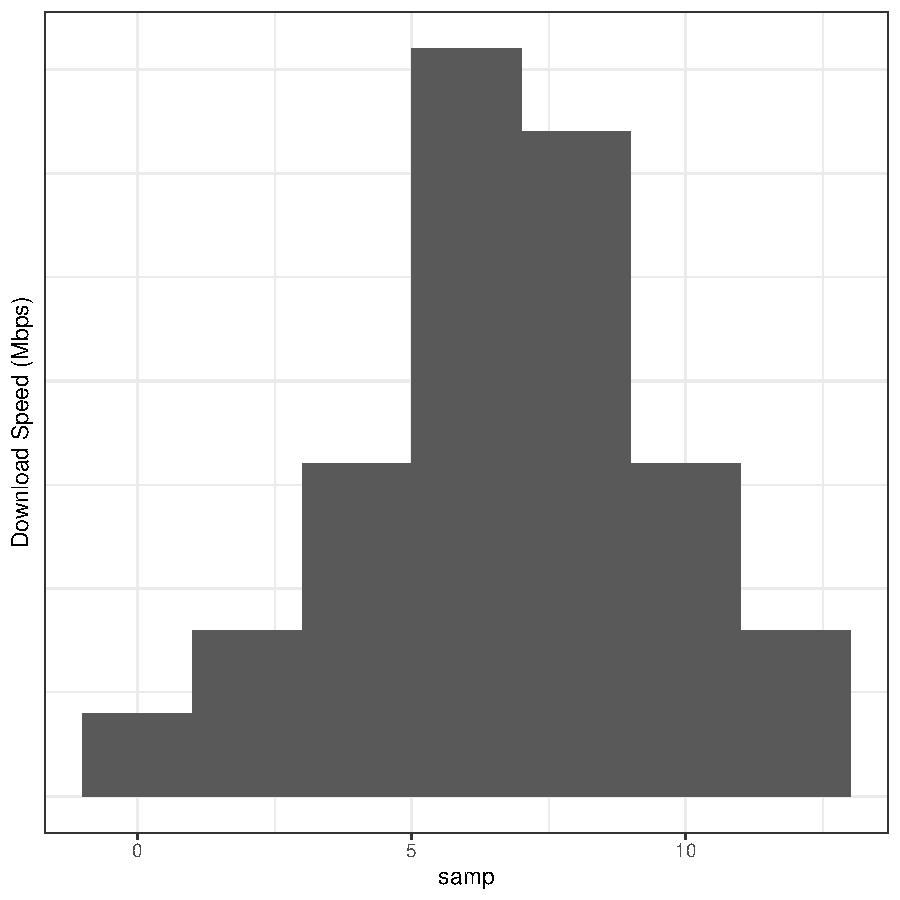
\includegraphics{stat305_hw2_sol-004}
  \item Create a box plot to summarize the data. Carefully label the axes.[10 pts]\\
  \emph{Solution:}
%-- : R code (Code in Document)
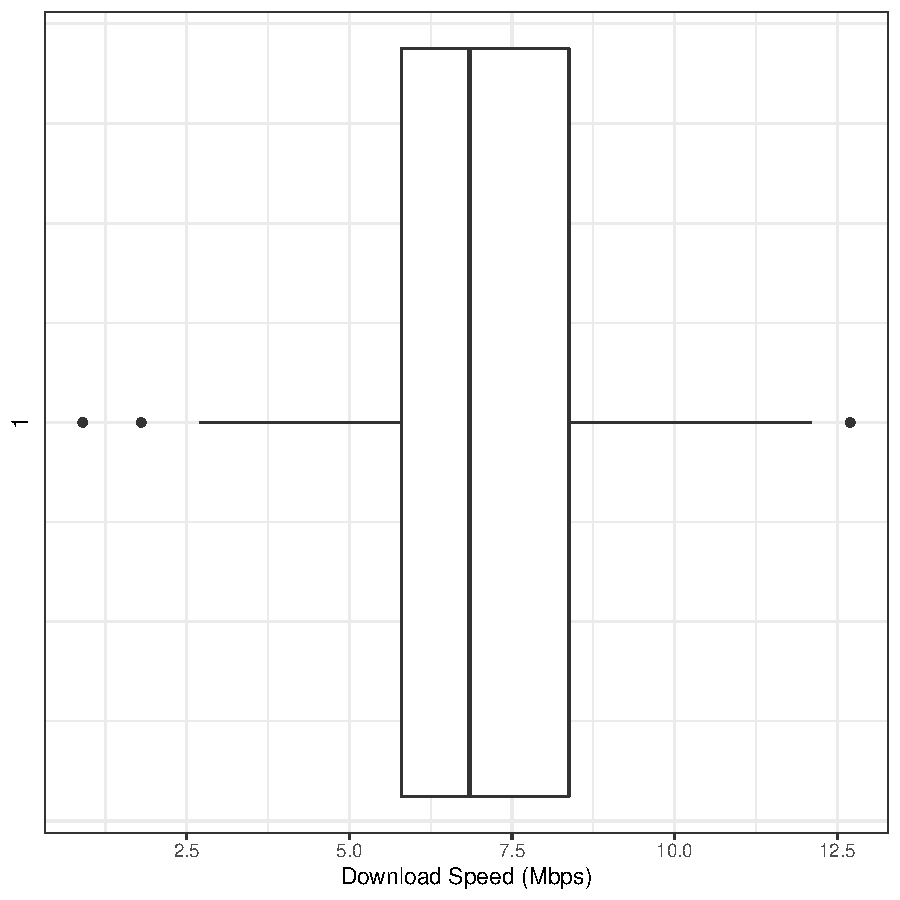
\includegraphics{stat305_hw2_sol-005}
Please note: the values on the y-axis are meaningless in this example. 
  \item Are there any unusually low observations? If so what were the speeds for those observations?[5 pts]\\
  \emph{Solution:} Yes, there are two unusually low observations as indicated by the box plot. 
     They had download speeds of at 0.9 Mbps and 1.8 Mbps.
     There is also one unusually high observations as indicated by the box plot. 
     It had download speeds of 12.7 Mbps.


  % \part[10] She also measured upload speed, obtaining the following 8 values.

%-- : R code (Code in Document)

% \begin{center}
%    7.45, 4.22, 7.7, 6.04, 7.68, 5.71, 4.71, 8.44
% \end{center}

% Create a theoretical Q-Q plot using the following quantiles from the normal distribution as the theoretical quantiles. Carefully label your axes.
% What does this graph tell us about the upload speeds?

% \begin{table}[h!]
%    \centering
%    \begin{tabular}{ccccccccc}
%              & 1 & 2 & 3 & 4 & 5 & 6 & 7 & 8 \\ \hline
%       $p$    & 0.0625 & 0.1875 & 0.3125 & 0.4375 & 0.5625 & 0.6875 & 0.8125 & 0.9375 \\
%       $Q(p)$ & -1.53 & -0.89 & -0.49 & -0.16 & 0.16 & 0.49 & 0.89 & 1.53 \\ \hline
%    \end{tabular}
% \end{table}

\end{enumerate}

\item  \textbf{[Ch 3, Exercise 8, pg. 116]} The accompanying data are the times to failure (in millions of cycles) of high-speed turbine engine bearings made out of two different compounds. These were taking from "Analysis of Single Classification Experiments Based on Censored Samples from the Two-parameter Weibull Distribution" by J. I. McCool (*The Journal of Statistical Planning and Inference*, 1979).
    

\begin{center}
	\begin{tabular}{|ccccccccccc|}	
		\hline
		compound_1  & 3.03 & 5.53 & 5.60 & 9.30 & 9.92 & 12.51 & 12.95 & 15.21 & 16.04 & 16.84\\
		compound_2 & 3.19 & 4.26 & 4.47 & 4.53 & 4.67 & 4.69 & 5.78 & 6.79 & 9.37 & 12.75\\
		\hline
	\hline                 
	\end{tabular}
\end{center}

\begin{enumerate}
    \item Find the .84 quantile of the Compound 1 failure times.[5 pts]\\
    \emph{Solution:} Using the steps in the notes:\\
    
     \begin{table}[h!]
     \centering
     \begin{tabular}{|l|p{2cm}|p{3cm}|p{3cm}|}
        \hline
                    \textbf{i}      & \textbf{(i- 0.5)/n} & \textbf{$Q_{1}((i- 0.5)/n)$} & \textbf{$Q_{2}((i- 0.5)/n)$}  \\\hline \hline
                    &  &  &  \\
      1   &  0.05 & 3.03 & 3.19 \\

      2   &  0.15 & 5.53 & 4.26 \\

      3   &  0.25 & 5.6 & 4.47 \\

      4   &  0.35 & 9.30 & 4.53 \\

      5  &  0.45 & 9.92 & 4.67 \\

      6  &  0.55 & 12.51 & 4.69 \\

      7  &  0.65 & 12.95 & 5.78 \\
      
      8  &  0.75 & 15.21 & 6.79 \\
      
      9  &  0.85 & 16.04 & 9.37 \\
      
      10  &  0.95 & 16.84 & 12.75 \\
      \hline
     \end{tabular}
  \end{table}
  since `\(\lfloor 8.9 \rfloor = 8 \)` then `\(i = 8\)` 
     \begin{align*}
       Q(.84) &= x_i + (n \cdot p - i + .5) \cdot \left( x_{i+1} - x_i \right)  \\\\
             &= x_8 + (10 \cdot 0.84 - 8 + .5) \cdot \left( x_{8+1} - x_8 \right)  \\\\
             &= x_8 + (0.9) \cdot \left( x_{9} - x_8 \right)  \\\\
             &= 15.21 + (.9) \cdot \left( 16.04 - 15.21 \right)  \\\\
             &= 15.975
  \end{align*}
    \item Find the median of the Compound 1 data.[5 pts]\\
    \emph{Solution:} 
      since `\(\lfloor 5.5 \rfloor = 5 \)` then `\(i = 5\)` 
     \begin{align*}
       Q(.5) &= x_i + (n \cdot p - i + .5) \cdot \left( x_{i+1} - x_i \right)  \\\\
             &= x_5 + (10 \cdot 0.5 - 5 + .5) \cdot \left( x_{5+1} - x_5 \right)  \\\\
             &= x_5 + (0.5) \cdot \left( x_{6} - x_5 \right)  \\\\
             &= 9.92 + (.5) \cdot \left( 12.51 - 9.92 \right)  \\\\
             &= 11.215
  \end{align*}
    \item Find the first quartile and the third quartile of compound 2.[10 pts]\\
    \emph{Solution:} \\
    $Q_2(0.25)= 4.47$\\
    $Q_2(0.75)= 6.79$
    \item Find the .23 quantile of compound 2. [5 pts]\\
    \emph{Solution:} \\
          since `\(\lfloor 2.8 \rfloor = 2 \)` then `\(i = 2\)` 
     \begin{align*}
       Q(.23) &= x_i + (n \cdot p - i + .5) \cdot \left( x_{i+1} - x_i \right)  \\\\
             &= x_2 + (10 \cdot 0.23 - 2 + .5) \cdot \left( x_{2+1} - x_2 \right)  \\\\
             &= x_2 + (0.8) \cdot \left( x_{3} - x_2 \right)  \\\\
             &= 4.26 + (0.8) \cdot \left( 4.47 - 4.26 \right)  \\\\
             &= 4.428
  \end{align*}
    
    
\end{enumerate}    

\item \textbf{JMP Assignment.} 

   Computing is one of the most important parts of modern data analysis. A large part of data science simply wouldn't exist without the tools developed by scientists working at the intersections of computer science, mathematics, and statistics. 
   Because of that, there will inevitably be parts of this course where a statistical computing tools are needed. SAS and R are the two main languages used by statisticians, though Python, Julia, F\#, C++ and others are also common.
   SAS has a software called JMP ("Jump") that makes doing statistical analyses simpler - it is more powerful than Excel or your calculator but requires little in the sense of coding making the learning curve much lower. 
   We will be using it this semester. There are labs in Snedecor Hall with the software pre-installed, but it is free for students and I encourage you to download a copy for yourself using the link below.

   Download: \href{https://www.stat.iastate.edu/statistical-software}{https://www.stat.iastate.edu/statistical-software}

   In this problem, we will work through the tutorial found at \href{http://web.utk.edu/~cwiek/201Tutorials/}{http://web.utk.edu/$\sim$cwiek/201Tutorials/}. Download and install \texttt{JMP} or find a computer with it already installed. Once you have done this, complete the following sections from the the tutorial linked above. For each part, print and include the table or graph produced. (Note: You can save the plots/tables and combine them in a single document).

\emph{For the JMP exercise, you just need to reproduce the same results on the tutorial using the data set available in the tutorial page.}
   \begin{enumerate}
      \item Creating a JMP data table [5 pts]
      \item Histogram and Box Plot[5 pts]
      \item Stem and Leaf Plot[5 pts]
      \item Side-by-Side Box Plots[5 pts]
   \end{enumerate}



\emph{Total: 145 pts}
\end{document}
